%%%%%%%%%%%%%%%%%%%%%%%%%%%%%%%%%%%%%%%%%
% University Assignment Title Page 
% LaTeX Template
% Version 1.0 (27/12/12)
%
% This template has been downloaded from:
% http://www.LaTeXTemplates.com
%
% Original author:
% WikiBooks (http://en.wikibooks.org/wiki/LaTeX/Title_Creation)
%
% License:
% CC BY-NC-SA 3.0 (http://creativecommons.org/licenses/by-nc-sa/3.0/)
% 
% Instructions for using this template:
% This title page is capable of being compiled as is. This is not useful for 
% including it in another document. To do this, you have two options: 
%
% 1) Copy/paste everything between \begin{document} and \end{document} 
% starting at \begin{titlepage} and paste this into another LaTeX file where you 
% want your title page.
% OR
% 2) Remove everything outside the \begin{titlepage} and \end{titlepage} and 
% move this file to the same directory as the LaTeX file you wish to add it to. 
% Then add %%%%%%%%%%%%%%%%%%%%%%%%%%%%%%%%%%%%%%%%%
% University Assignment Title Page 
% LaTeX Template
% Version 1.0 (27/12/12)
%
% This template has been downloaded from:
% http://www.LaTeXTemplates.com
%
% Original author:
% WikiBooks (http://en.wikibooks.org/wiki/LaTeX/Title_Creation)
%
% License:
% CC BY-NC-SA 3.0 (http://creativecommons.org/licenses/by-nc-sa/3.0/)
% 
% Instructions for using this template:
% This title page is capable of being compiled as is. This is not useful for 
% including it in another document. To do this, you have two options: 
%
% 1) Copy/paste everything between \begin{document} and \end{document} 
% starting at \begin{titlepage} and paste this into another LaTeX file where you 
% want your title page.
% OR
% 2) Remove everything outside the \begin{titlepage} and \end{titlepage} and 
% move this file to the same directory as the LaTeX file you wish to add it to. 
% Then add %%%%%%%%%%%%%%%%%%%%%%%%%%%%%%%%%%%%%%%%%
% University Assignment Title Page 
% LaTeX Template
% Version 1.0 (27/12/12)
%
% This template has been downloaded from:
% http://www.LaTeXTemplates.com
%
% Original author:
% WikiBooks (http://en.wikibooks.org/wiki/LaTeX/Title_Creation)
%
% License:
% CC BY-NC-SA 3.0 (http://creativecommons.org/licenses/by-nc-sa/3.0/)
% 
% Instructions for using this template:
% This title page is capable of being compiled as is. This is not useful for 
% including it in another document. To do this, you have two options: 
%
% 1) Copy/paste everything between \begin{document} and \end{document} 
% starting at \begin{titlepage} and paste this into another LaTeX file where you 
% want your title page.
% OR
% 2) Remove everything outside the \begin{titlepage} and \end{titlepage} and 
% move this file to the same directory as the LaTeX file you wish to add it to. 
% Then add %%%%%%%%%%%%%%%%%%%%%%%%%%%%%%%%%%%%%%%%%
% University Assignment Title Page 
% LaTeX Template
% Version 1.0 (27/12/12)
%
% This template has been downloaded from:
% http://www.LaTeXTemplates.com
%
% Original author:
% WikiBooks (http://en.wikibooks.org/wiki/LaTeX/Title_Creation)
%
% License:
% CC BY-NC-SA 3.0 (http://creativecommons.org/licenses/by-nc-sa/3.0/)
% 
% Instructions for using this template:
% This title page is capable of being compiled as is. This is not useful for 
% including it in another document. To do this, you have two options: 
%
% 1) Copy/paste everything between \begin{document} and \end{document} 
% starting at \begin{titlepage} and paste this into another LaTeX file where you 
% want your title page.
% OR
% 2) Remove everything outside the \begin{titlepage} and \end{titlepage} and 
% move this file to the same directory as the LaTeX file you wish to add it to. 
% Then add \input{./title_page_1.tex} to your LaTeX file where you want your
% title page.
%
%%%%%%%%%%%%%%%%%%%%%%%%%%%%%%%%%%%%%%%%%
%\title{Title page with logo}
%----------------------------------------------------------------------------------------
%	PACKAGES AND OTHER DOCUMENT CONFIGURATIONS
%----------------------------------------------------------------------------------------

\documentclass[12pt]{article}
\usepackage[english]{babel}
\usepackage[utf8x]{inputenc}
\usepackage{amsmath}
\usepackage{graphicx}
\usepackage[colorinlistoftodos]{todonotes}

\begin{document}

\begin{titlepage}

\newcommand{\HRule}{\rule{\linewidth}{0.5mm}} % Defines a new command for the horizontal lines, change thickness here

\center % Center everything on the page
 
%----------------------------------------------------------------------------------------
%	HEADING SECTIONS
%----------------------------------------------------------------------------------------

\textsc{\LARGE Politenico di Milano}\\[1.5cm] % Name of your university/college
\textsc{\Large Dipartimento Elettronica, Informazione e Bioingegneria}\\[0.5cm] % Major heading such as course name
\textsc{\large HEAPLab Project Report}\\[0.5cm] % Minor heading such as course title

%----------------------------------------------------------------------------------------
%	TITLE SECTION
%----------------------------------------------------------------------------------------

\HRule \\[0.4cm]
{ \huge \bfseries Title}\\[0.4cm] % Title of your document
\HRule \\[1.5cm]
 
%----------------------------------------------------------------------------------------
%	AUTHOR SECTION
%----------------------------------------------------------------------------------------

\begin{minipage}{0.4\textwidth}
\begin{flushleft} \large
\emph{Author:}\\
John \textsc{Smith} % Your name
\end{flushleft}
\end{minipage}
~
\begin{minipage}{0.4\textwidth}
\begin{flushright} \large
\emph{Supervisor:} \\
Dr. Giusppe \textsc{Massari} % Supervisor's Name
\end{flushright}
\end{minipage}\\[2cm]

% If you don't want a supervisor, uncomment the two lines below and remove the section above
%\Large \emph{Author:}\\
%John \textsc{Smith}\\[3cm] % Your name

%----------------------------------------------------------------------------------------
%	DATE SECTION
%----------------------------------------------------------------------------------------

{\large \today}\\[2cm] % Date, change the \today to a set date if you want to be precise

%----------------------------------------------------------------------------------------
%	LOGO SECTION
%----------------------------------------------------------------------------------------


\includegraphics[width=100pt]{heaplogo.pdf}\\[1cm] % Include a department/university logo - this will require the graphicx package
 
%----------------------------------------------------------------------------------------

\vfill % Fill the rest of the page with whitespace

\end{titlepage}




\begin{abstract}
Your abstract. - Summarize your work.
\end{abstract}

\section{Introduction}

Your introduction goes here! Some examples of commonly used commands and features are listed below, to help you get started.

If you have a question, please use the support box in the bottom right of the screen to get in touch. 


\section{Design and Implementation}

\section{Experimental Results}

\section{Conclusions}


\section{Some \LaTeX{} Examples}
\label{sec:examples}

\subsection{Sections}

Use section and subsection commands to organize your document. \LaTeX{} handles all the formatting and numbering automatically. Use ref and label commands for cross-references.

\subsection{Comments}

Comments can be added to the margins of the document using the \todo{Here's a comment in the margin!} todo command, as shown in the example on the right. You can also add inline comments too:

\todo[inline, color=green!40]{This is an inline comment.}

\subsection{Tables and Figures}

Use the table and tabular commands for basic tables --- see Table~\ref{tab:widgets}, for example. You can upload a figure (JPEG, PNG or PDF) using the files menu. To include it in your document, use the includegraphics command as in the code for Figure~\ref{fig:frog} below.

% Commands to include a figure:
\begin{figure}
\centering
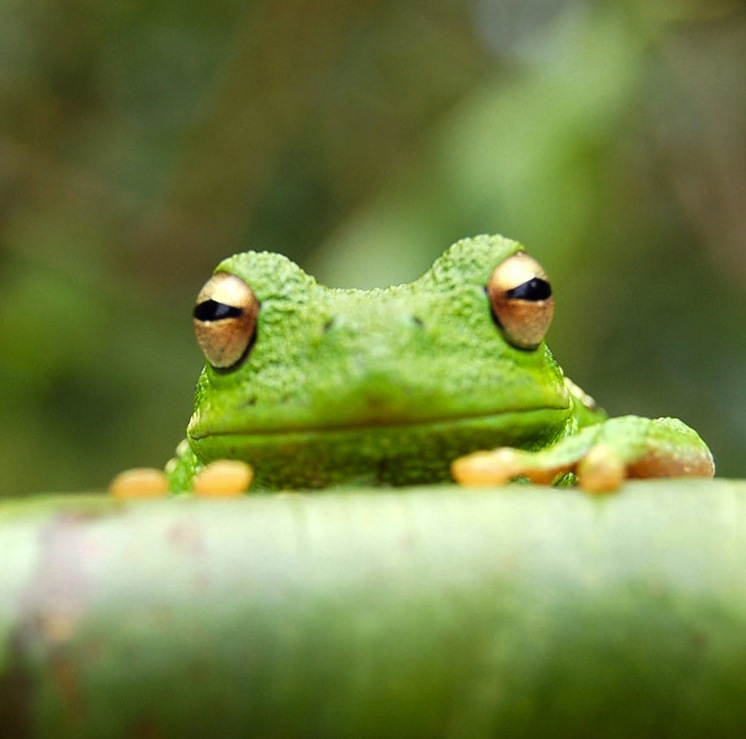
\includegraphics[width=0.5\textwidth]{frog.jpg}
\caption{\label{fig:frog}This is a figure caption.}
\end{figure}

\begin{table}
\centering
\begin{tabular}{l|r}
Item & Quantity \\\hline
Widgets & 42 \\
Gadgets & 13
\end{tabular}
\caption{\label{tab:widgets}An example table.}
\end{table}

\subsection{Mathematics}

\LaTeX{} is great at typesetting mathematics. Let $X_1, X_2, \ldots, X_n$ be a sequence of independent and identically distributed random variables with $\text{E}[X_i] = \mu$ and $\text{Var}[X_i] = \sigma^2 < \infty$, and let
$$S_n = \frac{X_1 + X_2 + \cdots + X_n}{n}
      = \frac{1}{n}\sum_{i}^{n} X_i$$
denote their mean. Then as $n$ approaches infinity, the random variables $\sqrt{n}(S_n - \mu)$ converge in distribution to a normal $\mathcal{N}(0, \sigma^2)$.

\subsection{Lists}

You can make lists with automatic numbering \dots

\begin{enumerate}
\item Like this,
\item and like this.
\end{enumerate}
\dots or bullet points \dots
\begin{itemize}
\item Like this,
\item and like this.
\end{itemize}

We hope you find write\LaTeX\ useful, and please let us know if you have any feedback using the help menu above.

\end{document} to your LaTeX file where you want your
% title page.
%
%%%%%%%%%%%%%%%%%%%%%%%%%%%%%%%%%%%%%%%%%
%\title{Title page with logo}
%----------------------------------------------------------------------------------------
%	PACKAGES AND OTHER DOCUMENT CONFIGURATIONS
%----------------------------------------------------------------------------------------

\documentclass[12pt]{article}
\usepackage[english]{babel}
\usepackage[utf8x]{inputenc}
\usepackage{amsmath}
\usepackage{graphicx}
\usepackage[colorinlistoftodos]{todonotes}

\begin{document}

\begin{titlepage}

\newcommand{\HRule}{\rule{\linewidth}{0.5mm}} % Defines a new command for the horizontal lines, change thickness here

\center % Center everything on the page
 
%----------------------------------------------------------------------------------------
%	HEADING SECTIONS
%----------------------------------------------------------------------------------------

\textsc{\LARGE Politenico di Milano}\\[1.5cm] % Name of your university/college
\textsc{\Large Dipartimento Elettronica, Informazione e Bioingegneria}\\[0.5cm] % Major heading such as course name
\textsc{\large HEAPLab Project Report}\\[0.5cm] % Minor heading such as course title

%----------------------------------------------------------------------------------------
%	TITLE SECTION
%----------------------------------------------------------------------------------------

\HRule \\[0.4cm]
{ \huge \bfseries Title}\\[0.4cm] % Title of your document
\HRule \\[1.5cm]
 
%----------------------------------------------------------------------------------------
%	AUTHOR SECTION
%----------------------------------------------------------------------------------------

\begin{minipage}{0.4\textwidth}
\begin{flushleft} \large
\emph{Author:}\\
John \textsc{Smith} % Your name
\end{flushleft}
\end{minipage}
~
\begin{minipage}{0.4\textwidth}
\begin{flushright} \large
\emph{Supervisor:} \\
Dr. Giusppe \textsc{Massari} % Supervisor's Name
\end{flushright}
\end{minipage}\\[2cm]

% If you don't want a supervisor, uncomment the two lines below and remove the section above
%\Large \emph{Author:}\\
%John \textsc{Smith}\\[3cm] % Your name

%----------------------------------------------------------------------------------------
%	DATE SECTION
%----------------------------------------------------------------------------------------

{\large \today}\\[2cm] % Date, change the \today to a set date if you want to be precise

%----------------------------------------------------------------------------------------
%	LOGO SECTION
%----------------------------------------------------------------------------------------


\includegraphics[width=100pt]{heaplogo.pdf}\\[1cm] % Include a department/university logo - this will require the graphicx package
 
%----------------------------------------------------------------------------------------

\vfill % Fill the rest of the page with whitespace

\end{titlepage}




\begin{abstract}
Your abstract. - Summarize your work.
\end{abstract}

\section{Introduction}

Your introduction goes here! Some examples of commonly used commands and features are listed below, to help you get started.

If you have a question, please use the support box in the bottom right of the screen to get in touch. 


\section{Design and Implementation}

\section{Experimental Results}

\section{Conclusions}


\section{Some \LaTeX{} Examples}
\label{sec:examples}

\subsection{Sections}

Use section and subsection commands to organize your document. \LaTeX{} handles all the formatting and numbering automatically. Use ref and label commands for cross-references.

\subsection{Comments}

Comments can be added to the margins of the document using the \todo{Here's a comment in the margin!} todo command, as shown in the example on the right. You can also add inline comments too:

\todo[inline, color=green!40]{This is an inline comment.}

\subsection{Tables and Figures}

Use the table and tabular commands for basic tables --- see Table~\ref{tab:widgets}, for example. You can upload a figure (JPEG, PNG or PDF) using the files menu. To include it in your document, use the includegraphics command as in the code for Figure~\ref{fig:frog} below.

% Commands to include a figure:
\begin{figure}
\centering
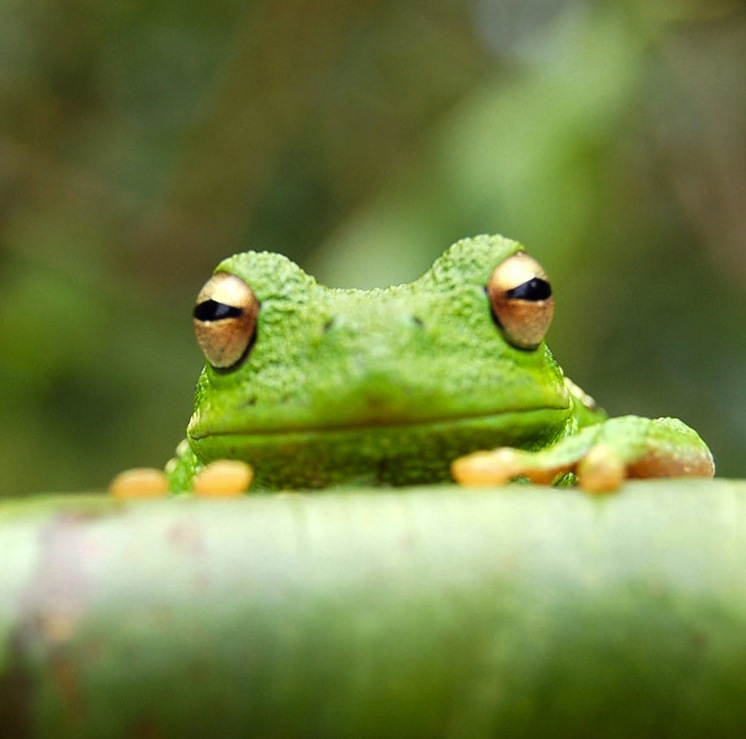
\includegraphics[width=0.5\textwidth]{frog.jpg}
\caption{\label{fig:frog}This is a figure caption.}
\end{figure}

\begin{table}
\centering
\begin{tabular}{l|r}
Item & Quantity \\\hline
Widgets & 42 \\
Gadgets & 13
\end{tabular}
\caption{\label{tab:widgets}An example table.}
\end{table}

\subsection{Mathematics}

\LaTeX{} is great at typesetting mathematics. Let $X_1, X_2, \ldots, X_n$ be a sequence of independent and identically distributed random variables with $\text{E}[X_i] = \mu$ and $\text{Var}[X_i] = \sigma^2 < \infty$, and let
$$S_n = \frac{X_1 + X_2 + \cdots + X_n}{n}
      = \frac{1}{n}\sum_{i}^{n} X_i$$
denote their mean. Then as $n$ approaches infinity, the random variables $\sqrt{n}(S_n - \mu)$ converge in distribution to a normal $\mathcal{N}(0, \sigma^2)$.

\subsection{Lists}

You can make lists with automatic numbering \dots

\begin{enumerate}
\item Like this,
\item and like this.
\end{enumerate}
\dots or bullet points \dots
\begin{itemize}
\item Like this,
\item and like this.
\end{itemize}

We hope you find write\LaTeX\ useful, and please let us know if you have any feedback using the help menu above.

\end{document} to your LaTeX file where you want your
% title page.
%
%%%%%%%%%%%%%%%%%%%%%%%%%%%%%%%%%%%%%%%%%
%\title{Title page with logo}
%----------------------------------------------------------------------------------------
%	PACKAGES AND OTHER DOCUMENT CONFIGURATIONS
%----------------------------------------------------------------------------------------

\documentclass[12pt]{article}
\usepackage[english]{babel}
\usepackage[utf8x]{inputenc}
\usepackage{amsmath}
\usepackage{graphicx}
\usepackage[colorinlistoftodos]{todonotes}

\begin{document}

\begin{titlepage}

\newcommand{\HRule}{\rule{\linewidth}{0.5mm}} % Defines a new command for the horizontal lines, change thickness here

\center % Center everything on the page
 
%----------------------------------------------------------------------------------------
%	HEADING SECTIONS
%----------------------------------------------------------------------------------------

\textsc{\LARGE Politenico di Milano}\\[1.5cm] % Name of your university/college
\textsc{\Large Dipartimento Elettronica, Informazione e Bioingegneria}\\[0.5cm] % Major heading such as course name
\textsc{\large HEAPLab Project Report}\\[0.5cm] % Minor heading such as course title

%----------------------------------------------------------------------------------------
%	TITLE SECTION
%----------------------------------------------------------------------------------------

\HRule \\[0.4cm]
{ \huge \bfseries Title}\\[0.4cm] % Title of your document
\HRule \\[1.5cm]
 
%----------------------------------------------------------------------------------------
%	AUTHOR SECTION
%----------------------------------------------------------------------------------------

\begin{minipage}{0.4\textwidth}
\begin{flushleft} \large
\emph{Author:}\\
John \textsc{Smith} % Your name
\end{flushleft}
\end{minipage}
~
\begin{minipage}{0.4\textwidth}
\begin{flushright} \large
\emph{Supervisor:} \\
Dr. Giusppe \textsc{Massari} % Supervisor's Name
\end{flushright}
\end{minipage}\\[2cm]

% If you don't want a supervisor, uncomment the two lines below and remove the section above
%\Large \emph{Author:}\\
%John \textsc{Smith}\\[3cm] % Your name

%----------------------------------------------------------------------------------------
%	DATE SECTION
%----------------------------------------------------------------------------------------

{\large \today}\\[2cm] % Date, change the \today to a set date if you want to be precise

%----------------------------------------------------------------------------------------
%	LOGO SECTION
%----------------------------------------------------------------------------------------


\includegraphics[width=100pt]{heaplogo.pdf}\\[1cm] % Include a department/university logo - this will require the graphicx package
 
%----------------------------------------------------------------------------------------

\vfill % Fill the rest of the page with whitespace

\end{titlepage}




\begin{abstract}
Your abstract. - Summarize your work.
\end{abstract}

\section{Introduction}

Your introduction goes here! Some examples of commonly used commands and features are listed below, to help you get started.

If you have a question, please use the support box in the bottom right of the screen to get in touch. 


\section{Design and Implementation}

\section{Experimental Results}

\section{Conclusions}


\section{Some \LaTeX{} Examples}
\label{sec:examples}

\subsection{Sections}

Use section and subsection commands to organize your document. \LaTeX{} handles all the formatting and numbering automatically. Use ref and label commands for cross-references.

\subsection{Comments}

Comments can be added to the margins of the document using the \todo{Here's a comment in the margin!} todo command, as shown in the example on the right. You can also add inline comments too:

\todo[inline, color=green!40]{This is an inline comment.}

\subsection{Tables and Figures}

Use the table and tabular commands for basic tables --- see Table~\ref{tab:widgets}, for example. You can upload a figure (JPEG, PNG or PDF) using the files menu. To include it in your document, use the includegraphics command as in the code for Figure~\ref{fig:frog} below.

% Commands to include a figure:
\begin{figure}
\centering
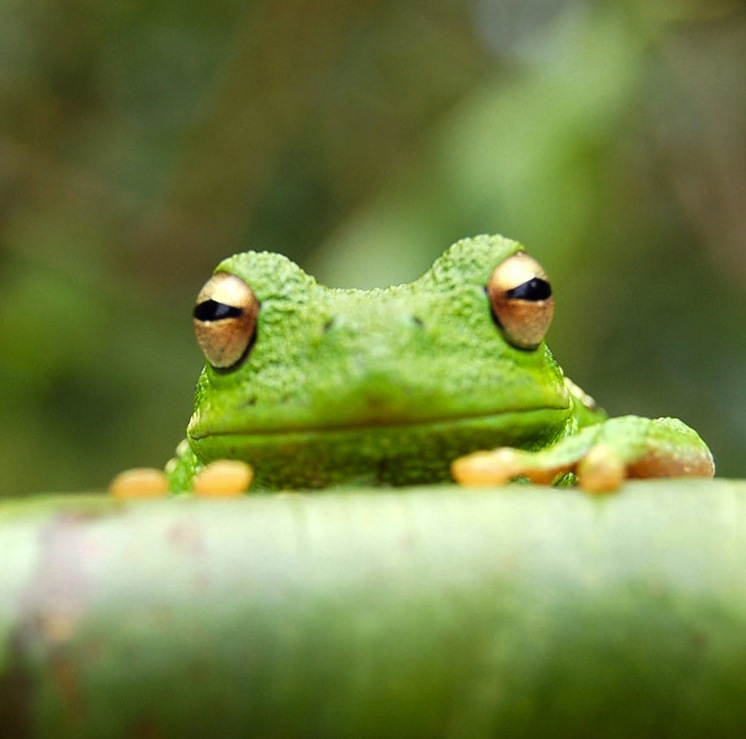
\includegraphics[width=0.5\textwidth]{frog.jpg}
\caption{\label{fig:frog}This is a figure caption.}
\end{figure}

\begin{table}
\centering
\begin{tabular}{l|r}
Item & Quantity \\\hline
Widgets & 42 \\
Gadgets & 13
\end{tabular}
\caption{\label{tab:widgets}An example table.}
\end{table}

\subsection{Mathematics}

\LaTeX{} is great at typesetting mathematics. Let $X_1, X_2, \ldots, X_n$ be a sequence of independent and identically distributed random variables with $\text{E}[X_i] = \mu$ and $\text{Var}[X_i] = \sigma^2 < \infty$, and let
$$S_n = \frac{X_1 + X_2 + \cdots + X_n}{n}
      = \frac{1}{n}\sum_{i}^{n} X_i$$
denote their mean. Then as $n$ approaches infinity, the random variables $\sqrt{n}(S_n - \mu)$ converge in distribution to a normal $\mathcal{N}(0, \sigma^2)$.

\subsection{Lists}

You can make lists with automatic numbering \dots

\begin{enumerate}
\item Like this,
\item and like this.
\end{enumerate}
\dots or bullet points \dots
\begin{itemize}
\item Like this,
\item and like this.
\end{itemize}

We hope you find write\LaTeX\ useful, and please let us know if you have any feedback using the help menu above.

\end{document} to your LaTeX file where you want your
% title page.
%
%%%%%%%%%%%%%%%%%%%%%%%%%%%%%%%%%%%%%%%%%
%\title{Title page with logo}
%----------------------------------------------------------------------------------------
%	PACKAGES AND OTHER DOCUMENT CONFIGURATIONS
%----------------------------------------------------------------------------------------

\documentclass[12pt]{article}
\usepackage[english]{babel}
\usepackage[utf8x]{inputenc}
\usepackage{amsmath}
\usepackage{graphicx}
\usepackage{listings}
\usepackage[colorinlistoftodos]{todonotes}
\usepackage{listings} 
\usepackage{multirow}
\usepackage{booktabs}


\begin{document}

\begin{titlepage}

\newcommand{\HRule}{\rule{\linewidth}{0.5mm}} % Defines a new command for the horizontal lines, change thickness here

\center % Center everything on the page
 
%----------------------------------------------------------------------------------------
%	HEADING SECTIONS
%----------------------------------------------------------------------------------------

\textsc{\LARGE Politenico di Milano}\\[1.5cm] % Name of your university/college
\textsc{\Large Dipartimento Elettronica, Informazione e Bioingegneria}\\[0.5cm] % Major heading such as course name
\textsc{\large HEAPLab Project Report}\\[0.5cm] % Minor heading such as course title

%----------------------------------------------------------------------------------------
%	TITLE SECTION
%----------------------------------------------------------------------------------------

\HRule \\[0.4cm]
{ \huge \bfseries Performance Estimation for TAFFO via LLVM-MCA}\\[0.4cm] % Title of your document
\HRule \\[1.5cm]
 
%----------------------------------------------------------------------------------------
%	AUTHOR SECTION
%----------------------------------------------------------------------------------------

\begin{minipage}{0.4\textwidth}
\begin{flushleft} \large
\emph{Author:}\\
Marco \textsc{Prosdocimi} % Your name
\end{flushleft}
\end{minipage}
~
\begin{minipage}{0.4\textwidth}
\begin{flushright} \large
\emph{Supervisors:} \\
Stefano \textsc{Cherubin} % Supervisor's Name
Daniele \textsc{Cattaneo} % Supervisor's Name
\end{flushright}
\end{minipage}\\[2cm]

% If you don't want a supervisor, uncomment the two lines below and remove the section above
%\Large \emph{Author:}\\
%John \textsc{Smith}\\[3cm] % Your name

%----------------------------------------------------------------------------------------
%	DATE SECTION
%----------------------------------------------------------------------------------------

{\large \today}\\[2cm] % Date, change the \today to a set date if you want to be precise

%----------------------------------------------------------------------------------------
%	LOGO SECTION
%----------------------------------------------------------------------------------------


\includegraphics[width=100pt]{heaplogo.pdf}\\[1cm] % Include a department/university logo - this will require the graphicx package
 
%----------------------------------------------------------------------------------------

\vfill % Fill the rest of the page with whitespace

\end{titlepage}




\begin{abstract}

This project aims to use LLVM-MCA to compare the fixed-point code produced by TAFFO with the original floating-point code for all loops in a given program to obtain a static prediction of the possible speedups gained by TAFFO.\\
LLVM-MCA is a tool that simulates the inner behavior of the CPU to estimate the performance of a machine code snippet.\\
TAFFO is an autotuning framework, based on LLVM 8, which tries to replace floating-point operations with fixed-point operations as much as possible.

\end{abstract}

\section{Introduction}

The purpose of this project is to build a tool that, by using the LLVM compiler infrastructure, finds loop bodies in a C program, compiles them with and without TAFFO, and uses LLVM-MCA to check if TAFFO is able to improve the execution time.
The tool uses LLVM-MCA in order to have a static prediction of the possible speedup given by TAFFO. Up to now, possible speedups were measured only at run time.

\section{Design and Implementation}
The tool consists of two different parts: the Loop Finder and the LLVM-MCA analysis.

\subsection{Loop Finder}
The Loop Finder uses LLVM APIs to search loops in the code and then add an Assembly inline comment then the loop's header and to the exit block.
The Assembly comments are "LLVM-MCA-BEGIN" and "LLVM-MCA-END"; 
 LLVM-MCA uses them to identify the region of code to analyze.
In the event of nested loops, the Loop Finder marks only the innermost ones.
Before running Loop Finder, loops are transformed into their canonical form: the latter has a pre-header and a single exit block. To realize that, I used the Loop Simplify LLVM pass that runs before Loop Finder.
Unfortunately, even by using Loop Simplify, I was not always able to transform loops into a form that allows them to have a single exit block.\\
In the current version of the tool, these kinds of loops are skipped.

\subsection{LLVM-MCA analysis}

LLVM-MCA is a performance analysis tool that uses information available in LLVM (e.g. scheduling models) to statically measure the performance of machine code in a specific CPU.
I modified the main procedure of LLVM-MCA so that it can show the total machine cycle count for all marked regions. The original version of LLVM-MCA was designed to print different analyses for all different regions marked in the code.
Having a general estimate of machine cycles, instead of several evaluations for individual regions, will make it easier to evaluate a possible speedup.
In the file "llvm-mca-mod.c" I underlined the original LLVM-MCA code and the few lines that I have changed.


\subsection{Outline of the operation performed by the tool}
The execution of the tool follows these main steps:
\begin{enumerate}
\item By using clang, it compiles the code and emits two LLVM IR files.
\item To generate the TAFFO IR file, it runs all TAFFO passes, and then the Loop Finder pass.
\item To generate the non TAFFO IR file, it executes only the Loop Finder pass.
\item The two IR files are compiled using LLC.
\item The modified version of LLVM-MCA is used to compute the cycle count on both of the Assembly files
\item For both of the files, the tool prints the results of the analysis.
\end{enumerate}

\section{Experimental procedure and evaluation}
To validate the operation of the tool, I ran several benchmarks.
I performed the analysis using the tool on an AMD A8-6600K x86 64 bit CPU, and I compared the speedup statically estimated by the tool with the real speedup measured at run time.

\subsection{Polybench benchmarks}
PolyBench is a collection of benchmarks used to validate experimental compilers. It consists of 30 different tests which have a single loop that dominates all the execution times. \\
By looking at the results in table 2, it can be observed that the predictions are not very accurate.
This behavior could be due to the inability of LLVM-MCA to predict cache behavior.
In the future, it will be necessary to repeat the tests using machines without cache, such as some microcontrollers.


\subsection{AxBench benchmarks}

AxBench is a suite of benchmarks use to evaluate applications for approximate computing.
For these benchmarks, instead of using the shell script tool, I wrote a Makefile that compiles the code with and without TAFFO and generates two different assembly files.
Then I used the modified version of LLVM-MCA on both Assembly files to estimate the machine cycles.
Even in this case, the tool's previsions are not very accurate.
The biggest problem lies in the impossibility of the current version of the tool to analyze all kinds of loops, as expressed in section 2.1.

\begin{table}[ht]
\begin{center}
\caption{Comparison of the speedup predicted by the tool and the measured speedup for AxBench}
\vspace{0.5cm}
\begin{tabular}{ |c|c|c| } 
 \hline
Test Name & Predicted speedup & Real speedup \\
 \hline
  blackscholes & 0.747 & 1.176 \\
 \hline
  fft & 3.254 & 0.998 \\
 \hline
  jmeint & 1.130 & 0.629\\
 \hline
  sobel & 2.430 & 0.0639 \\
 \hline
  inversek2j & 2.300 & 0.995 \\
 \hline
 \end{tabular}
\end{center}
\end{table}

\newpage

\begin{table}
\begin{center}
\caption{Comparison of the speedup predict by the tool and the measured speedup for Polybench}
\vspace{0.2cm}
\begin{tabular}{ |c|c|c| } 
 \hline
Test Name & Predicted speedup & Real speedup \\
 \hline
 correlation.c & 0.885 & 1.840 \\
 \hline
  covariance.c & 0.8896 & 1.919 \\
 \hline
  2mm.c & 1.164 & 2.153 \\
 \hline
  3mm.c & 1.187 & 2.598 \\
 \hline
  atax.c & 0.985 & 2.248 \\
 \hline
  bicg.c & 1.016 & 1.807 \\
 \hline
  doitgen.c & 0.809 & 3.157 \\
 \hline
  mvt.c & 0.953 & 2.232 \\
 \hline
  gemm.c & 1.126 & 0.822\\
 \hline
  gemver.c & 1.021 & 1.268 \\
 \hline
  gesummv.c & 1.138 & 1.740 \\
 \hline
  symm.c & 0.953 & 1.076 \\
 \hline
  syr2k.c & 1.126 & 0.696 \\
 \hline
  syrk.c & 1.096 & 0.918 \\
 \hline
  trmm.c & 1.024 & 1.996 \\
 \hline
  cholesky.c & 1.027 & 2.925 \\
 \hline
  durbin.c & 0.786 & 0.991 \\
 \hline
  gramschmidt.c & 0.963 & 1.235 \\
 \hline
  lu.c & 1.026 & 1.277 \\
 \hline
  ludcmp.c & 0.861 & 0.826 \\
 \hline
  trisolv.c & 0.858 & 2.491 \\
 \hline
  deriche.c & 0.664 & 1.429 \\
 \hline
  floyd-warshall.c & 0.974 & 2.370 \\
 \hline
  nussinov.c & 0.867 & 1.130 \\
 \hline
  adi.c & 0.924 & 0.936 \\
 \hline
  fdtd-2d.c & 0.852 & 2.720 \\
 \hline
  heat-3d.c & 0.915 & 3.107 \\
 \hline
  jacobi-1d.c & 0.934 & 1.696 \\
 \hline
  jacobi-2d.c & 0.956 & 1.860 \\
 \hline
  seidel-2d.c & 0.886 & 3.123 \\
 \hline
\end{tabular}
\end{center}
\end{table}
\newpage


\section{Conclusions and future developments}

The tool I created is useful if used as a new component of the TAFFO tool's chain, but it certainly needs some improvements.
The challenge in managing some specific kinds of loops -- those that don't have a single exit block after the execution of Loop Simplify -- makes the tool not entirely usable.
In the future, it will be necessary to change the "Loop Extractor" LLVM pass in order to add support to these kinds of loops that are currently skipped.
This problem is presented in some AxBench; thus, not all benchmarks result are fully reliable yet.
The best results when using TAFFO is achieved with machines without FPU (Floating Point Unit). In the future, it will be useful to repeat all benchmarks in this type of machine.


\begin{table}
\section{\fontsize{12}{15}\selectfont Appendix A Machine cycles measured by using the tool}
\begin{center}
\caption{Machine cycles estimated by using the tool for Polybench benchmarks (MC means machine cycles)}
\vspace{0.2cm}
\begin{tabular}{ |c|c|c| } 
 \hline
Test Name & Total number of MC & Total number of MC with TAFFO \\
 \hline
 correlation.c & 11379 & 12851 \\
 \hline
  covariance.c & 7086 & 7910 \\
 \hline
  2mm.c & 18940 & 16261 \\
 \hline
  3mm.c & 20772 & 17490 \\
 \hline
  atax.c & 8660 & 8791 \\
 \hline
  bicg.c & 14088 & 13855 \\
 \hline
  doitgen.c & 11557 & 14282 \\
 \hline
  mvt.c & 10634 & 11150 \\
 \hline
  gemm.c & 13633 & 12105 \\
 \hline
  gemver.c & 10101 & 9892 \\
 \hline
  gesummv.c & 10776 & 9467 \\
 \hline
  symm.c & 12764 & 13384 \\
 \hline
  syr2k.c & 13609 & 12082 \\
 \hline
  syrk.c & 10509 & 9582 \\
 \hline
  trmm.c & 7641 & 7458 \\
 \hline
  cholesky.c & 10705 & 10425 \\
 \hline
  durbin.c & 4789 & 6089 \\
 \hline
  gramschmidt.c & 11949 & 12399 \\
 \hline
  lu.c & 10705 & 10425 \\
 \hline
  ludcmp.c & 13660 & 15862 \\
 \hline
  trisolv.c & 4884 & 5688 \\
 \hline
  deriche.c & 14938 & 22465 \\
 \hline
  floyd-warshall.c & 16627 & 17054 \\
 \hline
  nussinov.c & 8506 & 9807 \\
 \hline
  adi.c & 7968 & 8615 \\
 \hline
  fdtd-2d.c & 13527 & 15870 \\
 \hline
  heat-3d.c & 14331 & 15655 \\
 \hline
  jacobi-1d.c & 5874 & 6283 \\
 \hline
  jacobi-2d.c & 7883 & 8562 \\
 \hline
  seidel-2d.c & 8700 & 9811 \\
 \hline
\end{tabular}
\end{center}
\end{table}

\begin{table}[ht]
\begin{center}
\caption{Machine cycles estimated by using the tool for AxBench benchmarks (MC means machine cycles)}
\vspace{0.5cm}
\begin{tabular}{ |c|c|c| } 
 \hline
Test Name & Total number of MC & Total number of MC with TAFFO \\
 \hline
  Blackscholes & 6402 & 8571 \\
 \hline
  fft & 36718 & 11281 \\
 \hline
  jmeint & 1720 & 1521 \\
 \hline
  sobel & 27094 & 11149 \\
 \hline
  inversek2j & 102512 & 44571 \\
 \hline
 \end{tabular}
\end{center}
\end{table}

\end{document}